\section{Profile SCFG construction: the \texttt{cmbuild} program}
WR
\software{infernal} builds a model of consensus RNA secondary
structure using a formalism called a \emph{covariance model} (CM),
which is a type of \emph{profile stochastic context-free grammar}
(profile SCFG) \cite{Eddy94,Durbin98,Eddy02b}.

What follows is a technical description of what CM is, how it
corresponds to a known RNA secondary structure, and how it is built
and parameterized.\footnote{Much of this text is taken from
\cite{Eddy02b}.}  You certainly don't have to understand the technical
details of CMs to understand \prog{cmbuild} or \software{infernal},
but it will probably help to at least skim this part. After that is a
description of what the \prog{cmbuild} program does to build a CM from
an input RNA multiple alignment, and how to control the behavior of
the program.

\subsection{Technical description of a covariance model}

\subsubsection{Definition of a stochastic context free grammar}

A stochastic context free grammar (SCFG) consists of the following:

\begin{itemize}
\item $M$ different nonterminals (here called \emph{states}). I will use capital
      letters to refer to specific nonterminals; $V$ and $Y$ will be used
      to refer generically to unspecified nonterminals.
\item $K$ different terminal symbols (e.g. the observable alphabet,
      {a,c,g,u} for RNA). I will use small letters $a,b$ to refer
      generically to terminal symbols.
\item a number of \emph{production rules} of the form: $V \rightarrow
\gamma$, where $\gamma$ can be any string of nonterminal and/or
terminal symbols, including (as a special case) the empty string
$\epsilon$.
\item Each production rule is associated with a probability, such that
      the sum of the production probabilities for any given
      nonterminal $V$ is equal to 1.
\end{itemize} 

\subsubsection{SCFG productions allowed in CMs}

A CM is a specific, repetitive SCFG architecture consisting of groups
of model states that are associated with base pairs and
single-stranded positions in an RNA secondary structure consensus. A
CM has seven types of states and production rules:

\vspace{0.5em}
\begin{center}
\begin{tabular}{lllll}
State type & Description             &  Production             & Emission & Transition\\ \hline
P & (pair emitting)   & $P \rightarrow a Y b$ & $e_v(a,b)$ & $t_v(Y)$  \\
L & (left emitting)   & $L \rightarrow a Y$   & $e_v(a)$   & $t_v(Y)$  \\
R & (right emitting)  & $R \rightarrow Y a$   & $e_v(a)$   & $t_v(Y)$  \\
B & (bifurcation)     & $B \rightarrow S S$   & 1     &     1     \\
D & (delete)          & $D \rightarrow Y$     & 1     &   $t_v(Y)$  \\
S & (start)           & $S \rightarrow Y$     &    1     & $t_v(Y)$  \\
E & (end)             & $E \rightarrow \epsilon$ & 1     &     1     \\
\end{tabular}
\end{center}
\vspace{0.5em}

Each overall production probability is the independent product of an
emission probability $e_v$ and a transition probability $t_v$, both of
which are position-dependent parameters that depend on the state $v$
(analogous to hidden Markov models). For example, a particular pair
(P) state $v$ produces two correlated letters $a$ and $b$ (e.g. one of
16 possible base pairs) with probability $e_v(a,b)$ and transits to
one of several possible new states $Y$ of various types with
probability $t_v(Y)$.  A bifurcation (B) state splits into two new
start ($S$) states with probability 1.  The E state is a special case
$\epsilon$ production that terminates a derivation.

A CM consists of many states of these seven basic types, each with its
own emission and transition probability distributions, and its own set
of states that it can transition to. Consensus base pairs will be
modeled by P states, consensus single stranded residues by L and R
states, insertions relative to the consensus by more L and R states,
deletions relative to consensus by D states, and the branching
topology of the RNA secondary structure by B, S, and E states. The
procedure for starting from an input multiple alignment and
determining how many states, what types of states, and how they are
interconnected by transition probabilities is described next.

\subsubsection{From consensus structural alignment to guide tree}

Figure~\ref{fig:input_alignment} shows an example input file: a
multiple sequence alignment of homologous RNAs, with a line in WUSS
notation that describes the consensus RNA secondary structure. The
first step of building a CM is to produce a binary \emph{guide tree}
of \emph{nodes} representing the consensus secondary structure. The
guide tree is a parse tree for the consensus structure, with nodes as
nonterminals and alignment columns as terminals.

\begin{figure}[t]
\begin{center}
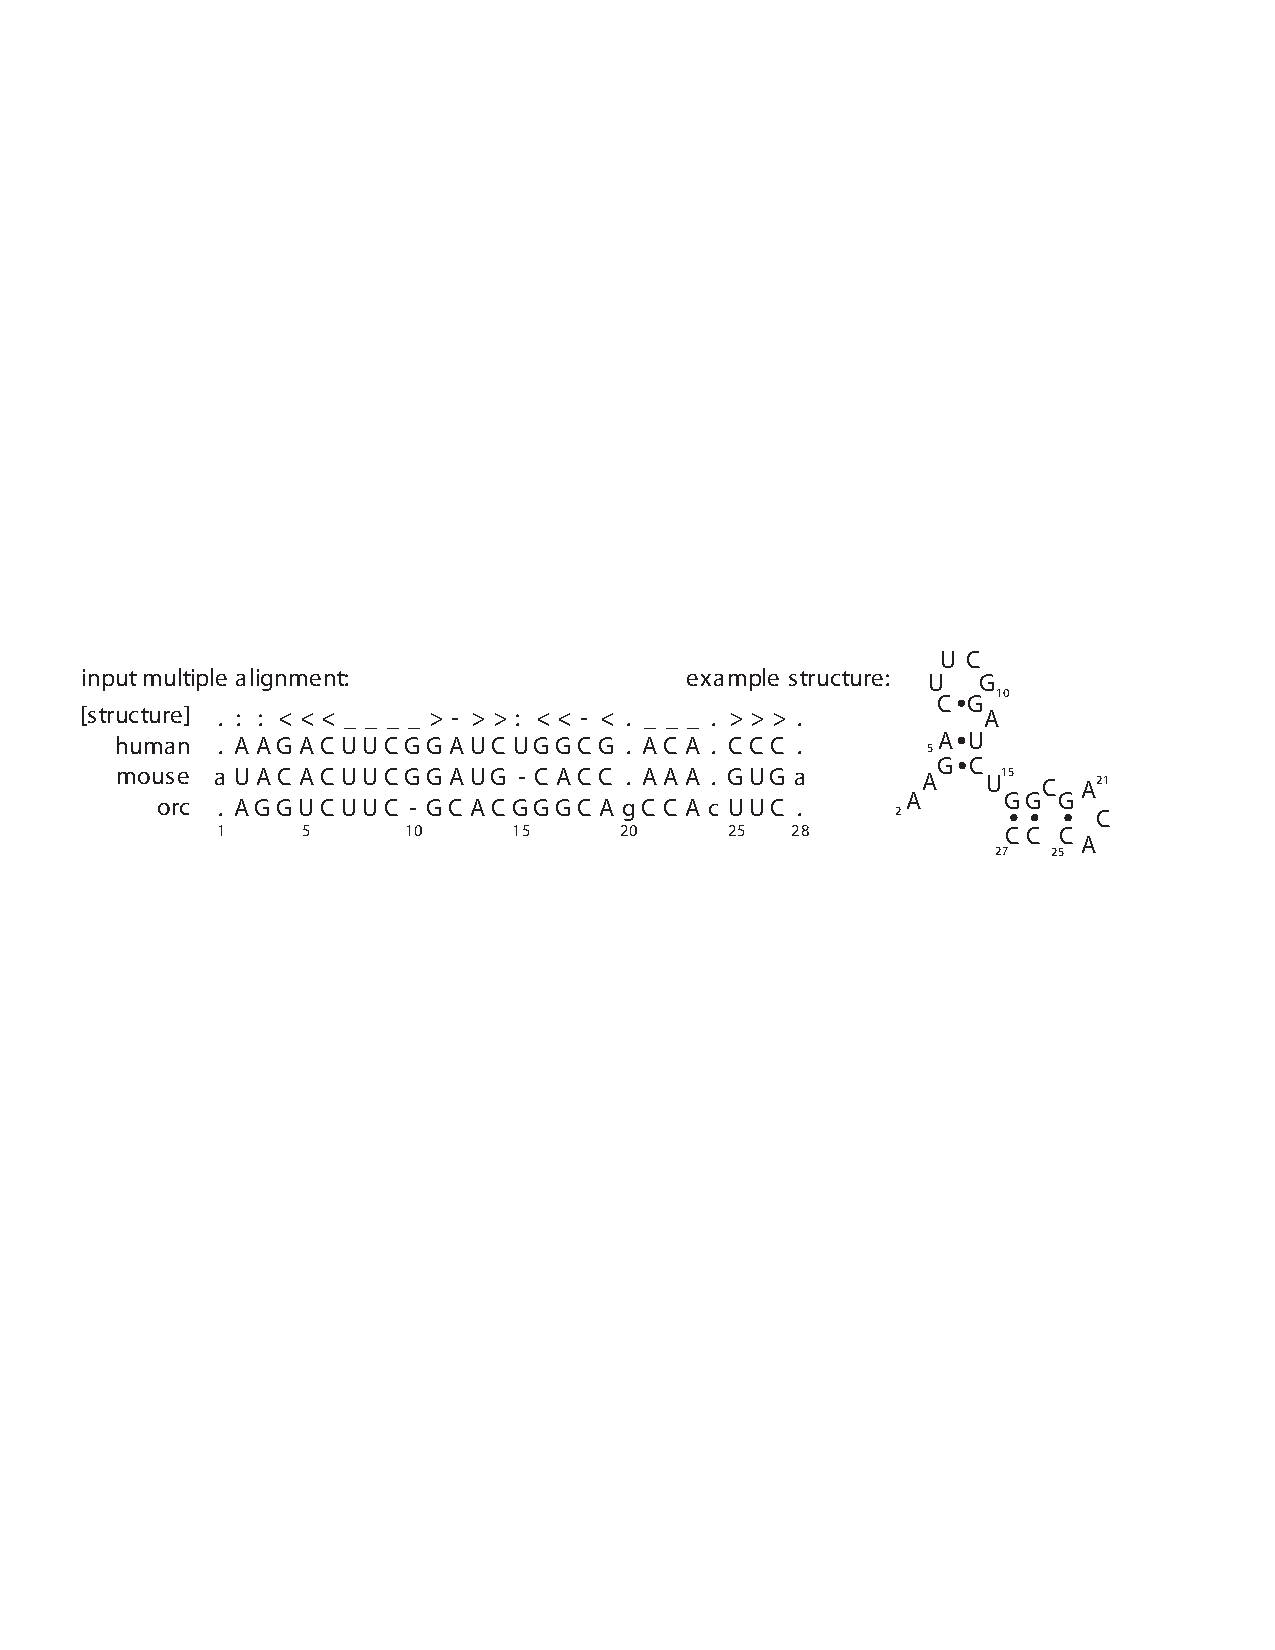
\includegraphics[scale=0.8]{Figures/input_alignment}
\end{center}
\caption{\small\textbf{An example RNA sequence family.} Left: a toy multiple
alignment of three sequences, with 28 total columns, 24 of which will
be modeled as consensus positions. The [structure] line annotates the
consensus secondary structure in WUSS notation.
Right: the secondary structure of the ``human'' sequence.} 
\label{fig:input_alignment}
\end{figure}

The guide tree has eight types of nodes:

\vspace{0.5em}
\begin{center}
\begin{tabular}{lll}
Node      & Description        &  Main state type          \\ \hline
MATP  & (pair)                 & P \\
MATL  & (single strand, left)  & L \\
MATR  & (single strand, right) & R \\
BIF   & (bifurcation)          & B \\
ROOT  & (root)                 & S \\
BEGL  & (begin, left)          & S \\
BEGR  & (begin, right)         & S \\
END   & (end)                  & E \\
\end{tabular}
\end{center}
\vspace{0.5em}
 
These consensus node types correspond closely with the CM's final
state types. Each node will eventually contain one or more states. The
guide tree deals with the consensus structure. For individual
sequences, we will need to deal with insertions and deletions with
respect to this consensus. The guide tree is the skeleton on which we
will organize the CM. For example, a MATP node will contain a P-type
state to model a consensus base pair; but it will also contain several
other states to model infrequent insertions and deletions at or
adjacent to this pair.

The input alignment is first used to construct a consensus secondary
structure (Figure~\ref{fig:cm_nodetree}) that defines which aligned
columns will be ignored as non-consensus (and later modeled as
insertions relative to the consensus), and which consensus alignment
columns are base-paired to each other. For the purposes of this
description, I assume that both the structural annotation and the
labeling of insert versus consensus columns is given in the input
file, as shown in the alignment in Figure~\ref{fig:input_alignment},
where both are are indicated by the WUSS notation in the [structure]
line (where, e.g., insert columns are marked with \verb+.+). (In
practice, \prog{cmbuild} does need secondary structure annotation, but
it doesn't require insert/consensus annotation or full WUSS notation
in its input alignment files; this would require a lot of manual
annotation.  More on this later.)

\begin{figure}[t]
\begin{center}
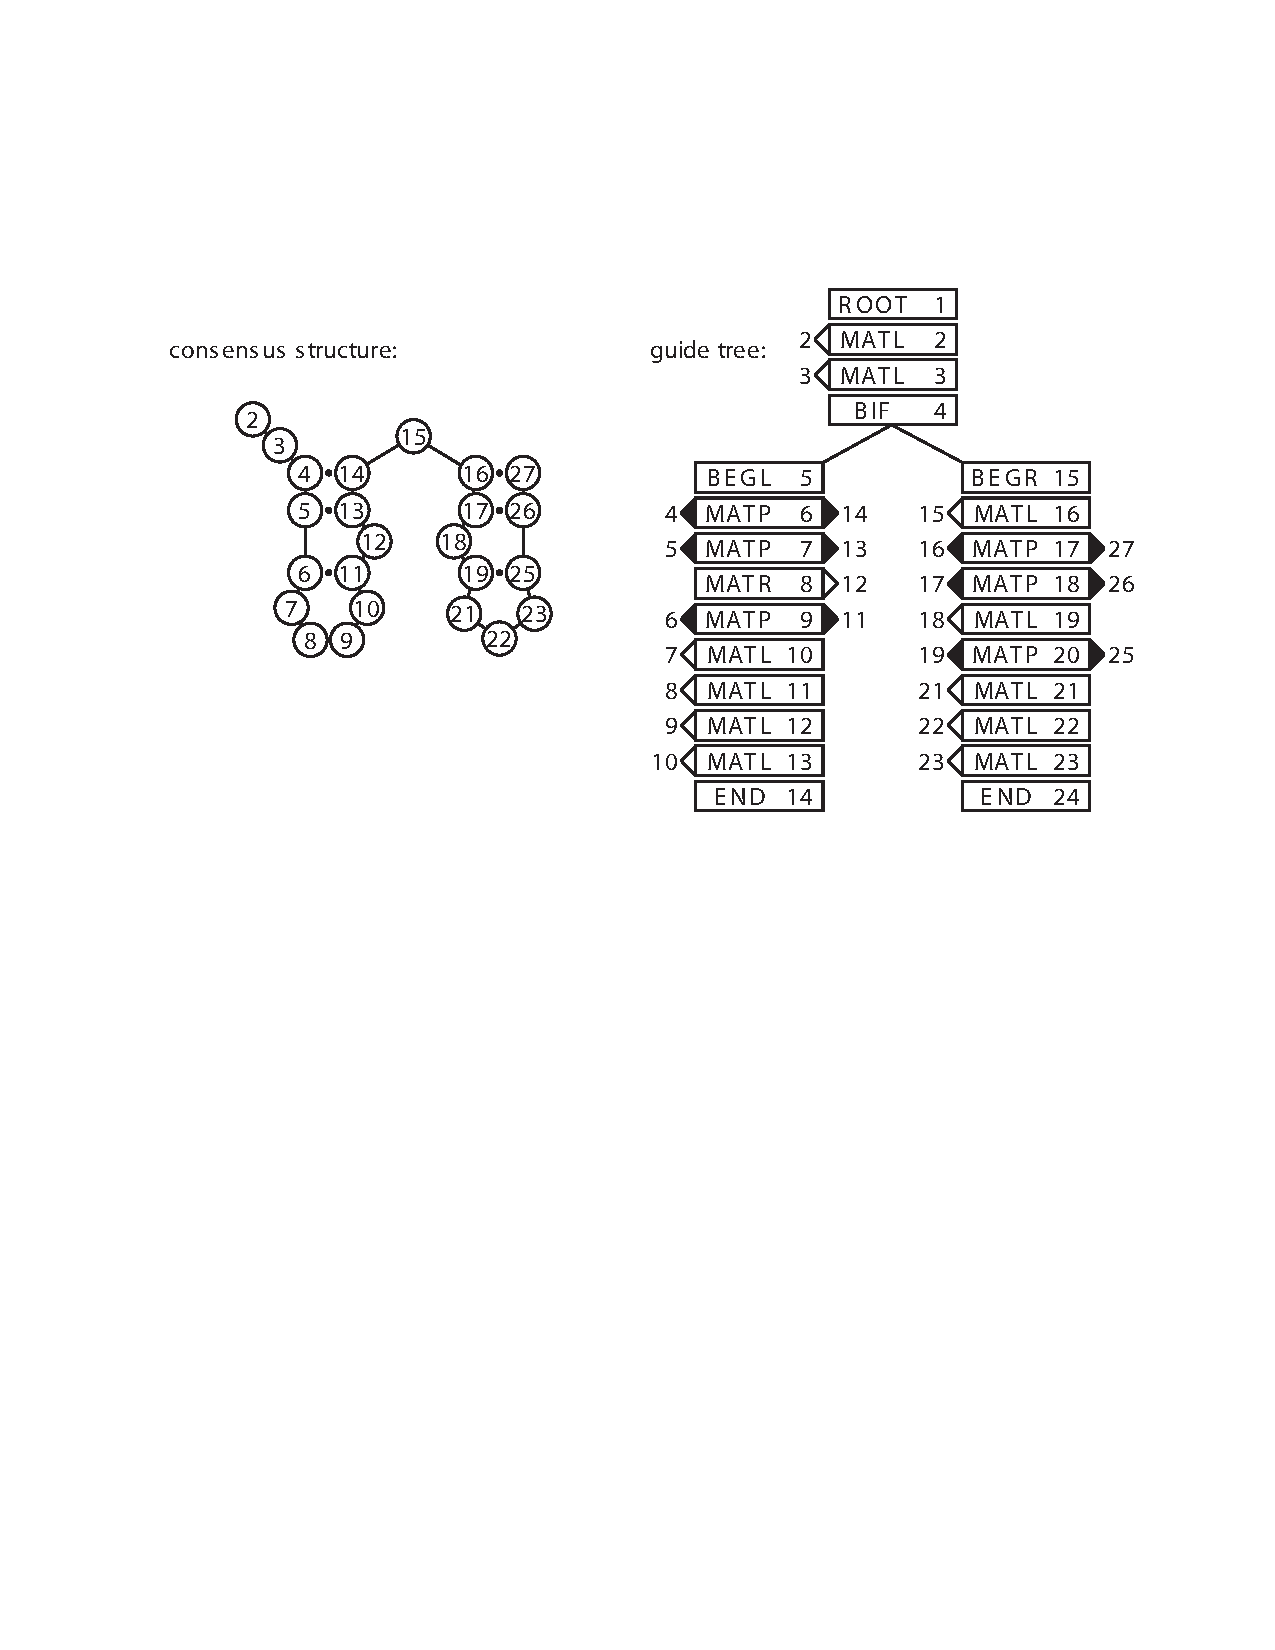
\includegraphics[width=5in]{Figures/cm_nodetree}
\end{center}
\caption{\small\textbf{The structural alignment is converted to a guide
tree.} Left: the consensus secondary structure is derived from the
annotated alignment in Figure~\ref{fig:input_alignment}. Numbers in
the circles indicate alignment column coordinates: e.g.  column 4 base
pairs with column 14, and so on. Right: the CM guide tree
corresponding to this consensus structure. The nodes of the tree are
numbered 1..24 in preorder traversal (see text). MATP, MATL, and MATR
nodes are associated with the columns they generate: e.g., node 6 is a
MATP (pair) node that is associated with the base-paired columns 4 and
14.}
\label{fig:cm_nodetree}
\end{figure}

Given the consensus structure, consensus base pairs are assigned to
MATP nodes and consensus unpaired columns are assigned to MATL or MATR
nodes. One ROOT node is used at the head of the tree.  Multifurcation
loops and/or multiple stems are dealt with by assigning one or more
BIF nodes that branch to subtrees starting with BEGL or BEGR head
nodes. (ROOT, BEGL, and BEGR start nodes are labeled differently
because they will be expanded to different groups of states; this has
to do with avoiding ambiguous parse trees for individual sequences, as
described below.) Alignment columns that are considered to be
insertions relative to the consensus structure are ignored at this
stage.

In general there will be more than one possible guide tree for any
given consensus structure. Almost all of this ambiguity is eliminated
by three conventions: (1) MATL nodes are always used instead of MATR
nodes where possible, for instance in hairpin loops; (2) in describing
interior loops, MATL nodes are used before MATR nodes; and (3) BIF
nodes are only invoked where necessary to explain branching secondary
structure stems (as opposed to unnecessarily bifurcating in single
stranded sequence). One source of ambiguity remains. In invoking a
bifurcation to explain alignment columns $i..j$ by two substructures
on columns $i..k$ and $k+1..j$, there will be more than one possible
choice of $k$ if $i..j$ is a multifurcation loop containing three or
more stems. The choice of $k$ impacts the performance of the divide
and conquer algorithm; for optimal time performance, we will want
bifurcations to split into roughly equal sized alignment problems, so
I choose the $k$ that makes $i..k$ and $k+1..j$ as close to the same
length as possible.

The result of this procedure is the guide tree. The nodes of the guide
tree are numbered in preorder traversal (e.g. a recursion of ``number
the current node, visit its left child, visit its right child'': thus
parent nodes always have lower indices than their children). The guide
tree corresponding to the input multiple alignment in
Figure~\ref{fig:input_alignment} is shown in
Figure~\ref{fig:cm_nodetree}.

\subsubsection{From guide tree to covariance model}

A CM must deal with insertions and deletions in individual sequences
relative to the consensus structure. For example, for a consensus base
pair, either partner may be deleted leaving a single unpaired residue,
or the pair may be entirely deleted; additionally, there may be
inserted nonconsensus residues between this pair and the next pair in
the stem. Accordingly, each node in the master tree is expanded into
one or more \emph{states} in the CM as follows:

\vspace{0.5em}
\begin{center}
\begin{tabular}{llccc}
       &                     & total \#& \# of split& \# of insert\\
Node   &  States             & states  & states     & states \\ \hline
MATP   & [MP ML MR D] IL IR  &   6     &   4        &  2   \\
MATL   & [ML D] IL           &   3     &   2    &  1   \\
MATR   & [MR D] IR           &   3     &   2    &  1   \\
BIF    & [B]                 &   1     &   1    &  0   \\
ROOT   & [S] IL IR           &   3     &   1    &  2   \\
BEGL   & [S]                 &   1     &   1    &  0   \\
BEGR   & [S] IL              &   2     &   1    &  1   \\
END    & [E]                 &   1     &   1    &  0   \\ \hline
\end{tabular}
\end{center}
\vspace{0.5em}

Here we distinguish between consensus (``M'', for ``match'') states
and insert (``I'') states. ML and IL, for example, are both L type
states with L type productions, but they will have slightly different
properties, as described below.

The states are grouped into a \emph{split set} of 1-4 states (shown in
brackets above) and an \emph{insert set} of 0-2 insert states. The
split set includes the main consensus state, which by convention is
first. One and only one of the states in the split set must be visited
in every parse tree (and this fact will be exploited by the divide and
conquer algorithm). The insert state(s) are not obligately visited,
and they have self-transitions, so they will be visited zero or more
times in any given parse tree.

State transitions are then assigned as follows. For bifurcation nodes,
the B state makes obligate transitions to the S states of the child
BEGL and BEGR nodes. For other nodes, each state in a split set has a
possible transition to every insert state in the \emph{same} node, and
to every state in the split set of the \emph{next} node. An IL state
makes a transition to itself, to the IR state in the same node (if
present), and to every state in the split set of the next node. An IR
state makes a transition to itself and to every state in the split set
of the next node.

This arrangement of transitions guarantees that (given the guide tree)
there is unambiguously one and only one parse tree for any given
individual structure. This is important. The algorithm will find a
maximum likelihood parse tree for a given sequence, and we wish to
interpret this result as a maximum likelihood structure, so there must
be a one to one relationship between parse trees and secondary
structures \cite{Giegerich00}.

The final CM is an array of $M$ states, connected as a directed graph
by transitions $t_v(y)$ (or probability 1 transitions $v \rightarrow
(y,z)$ for bifurcations) with the states numbered such that $(y,z)
\geq v$. There are no cycles in the directed graph other than cycles
of length one (e.g. the self-transitions of the insert states). We can
think of the CM as an array of states in which all transition
dependencies run in one direction; we can do an iterative dynamic
programming calculation through the model states starting with the
last numbered end state $M$ and ending in the root state $1$.  An
example CM, corresponding to the input alignment of
Figure~\ref{fig:input_alignment}, is shown in
Figure~\ref{fig:cm_graph}.

As a convenient side effect of the construction procedure, it is
guaranteed that the transitions from any state are to a
\emph{contiguous} set of child states, so the transitions for state
$v$ may be kept as an offset and a count. For example, in
Figure~\ref{fig:cm_graph}, state 12 (an MP) connects to states 16, 17,
18, 19, 20, and 21. We can store this as an offset of 4 to the first
connected state, and a total count of 6 connected states.  We know
that the offset is the distance to the next non-split state in the
current node; we also know that the count is equal to the number of
insert states in the current node, plus the number of split set states
in the next node. These properties make establishing the connectivity
of the CM trivial. Similarly, all the parents of any given state are
also contiguously numbered, and can be determined analogously. We are
also guaranteed that the states in a split set are numbered
contiguously.  This contiguity is exploited by the divide and conquer
implementation.

\begin{figure}[tp]
\begin{center}
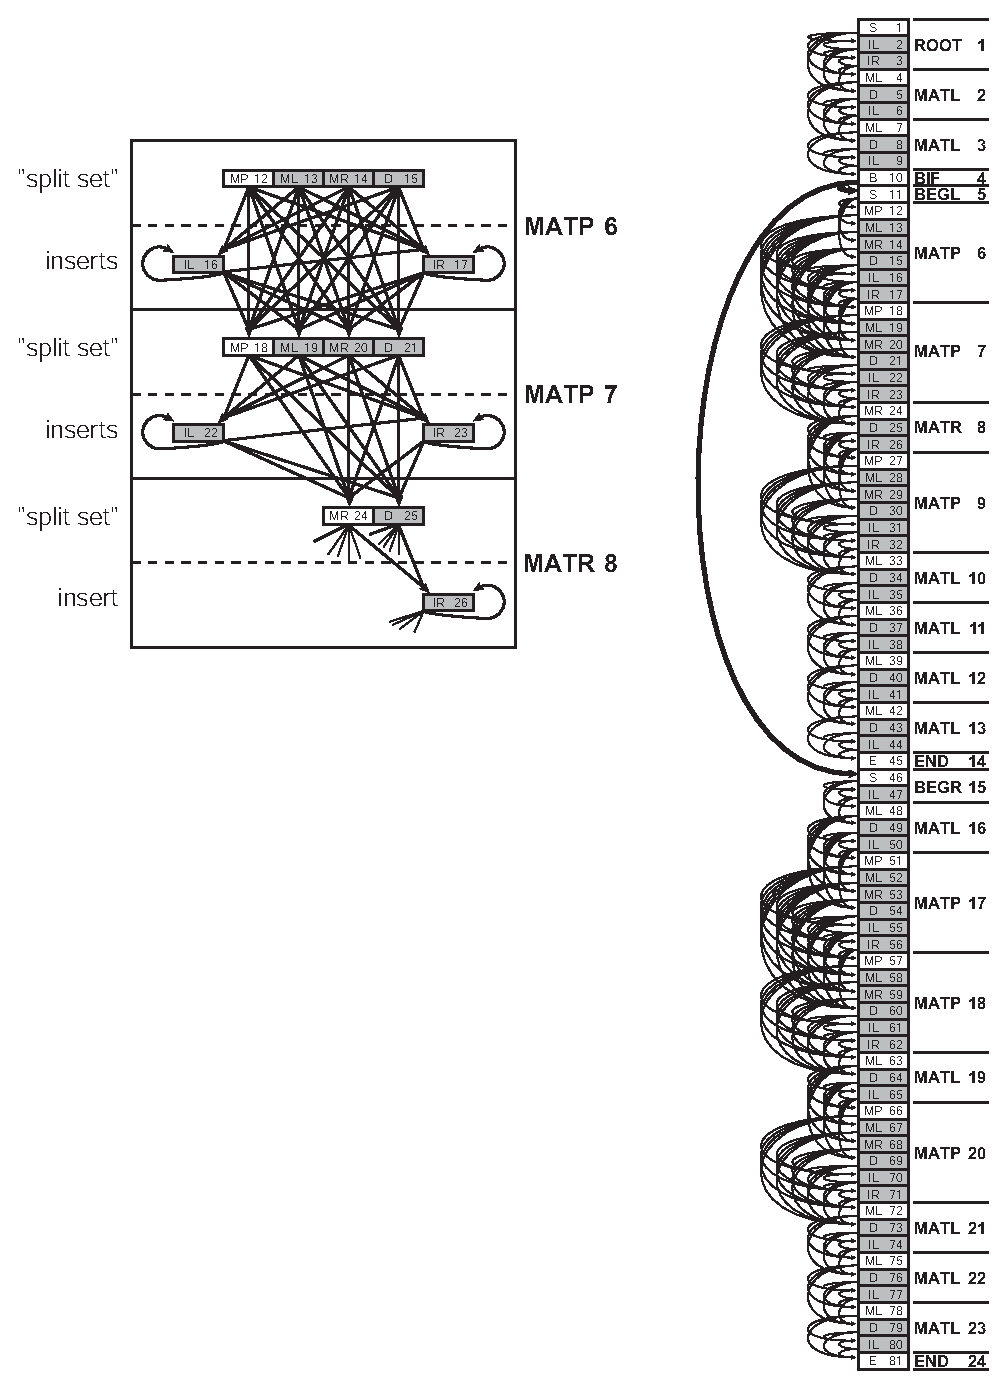
\includegraphics[width=5in]{Figures/cm_graph}
\end{center}
\caption{\small\textbf{A complete covariance model.} Right: the CM
corresponding to the alignment in Figure~\ref{fig:input_alignment}.
The model has 81 states (boxes, stacked in a vertical array). Each
state is associated with one of the 24 nodes of the guide tree (text
to the right of the state array). States corresponding to the
consensus are in white. States responsible for insertions and
deletions are gray. The transitions from bifurcation state B10 to
start states S11 and S46 are in bold because they are special: they
are an obligate (probability 1) bifurcation. All other transitions
(thin arrows) are associated with transition probabilities.  Emission
probability distributions are not represented in the figure. Left: the
states are also arranged according to the guide tree. A blow up of
part of the model corresponding to nodes 6, 7, and 8 shows
more clearly the logic of the connectivity of transition probabilities
(see main text), and also shows why any parse tree must transit through
one and only one state in each ``split set''.}
\label{fig:cm_graph}
\end{figure}

\subsubsection{Parameterization}

Using the guide tree and the final CM, each individual sequence in the
input multiple alignment can be converted unambiguously to a CM parse
tree, as shown in Figure~\ref{fig:parsetrees}. Weighted counts for
observed state transitions and singlet/pair emissions are then
collected from these parse trees. These counts are converted to
transition and emission probabilities, as maximum \emph{a posteriori}
estimates using mixture Dirichlet priors.

\begin{figure}[t]
\begin{center}
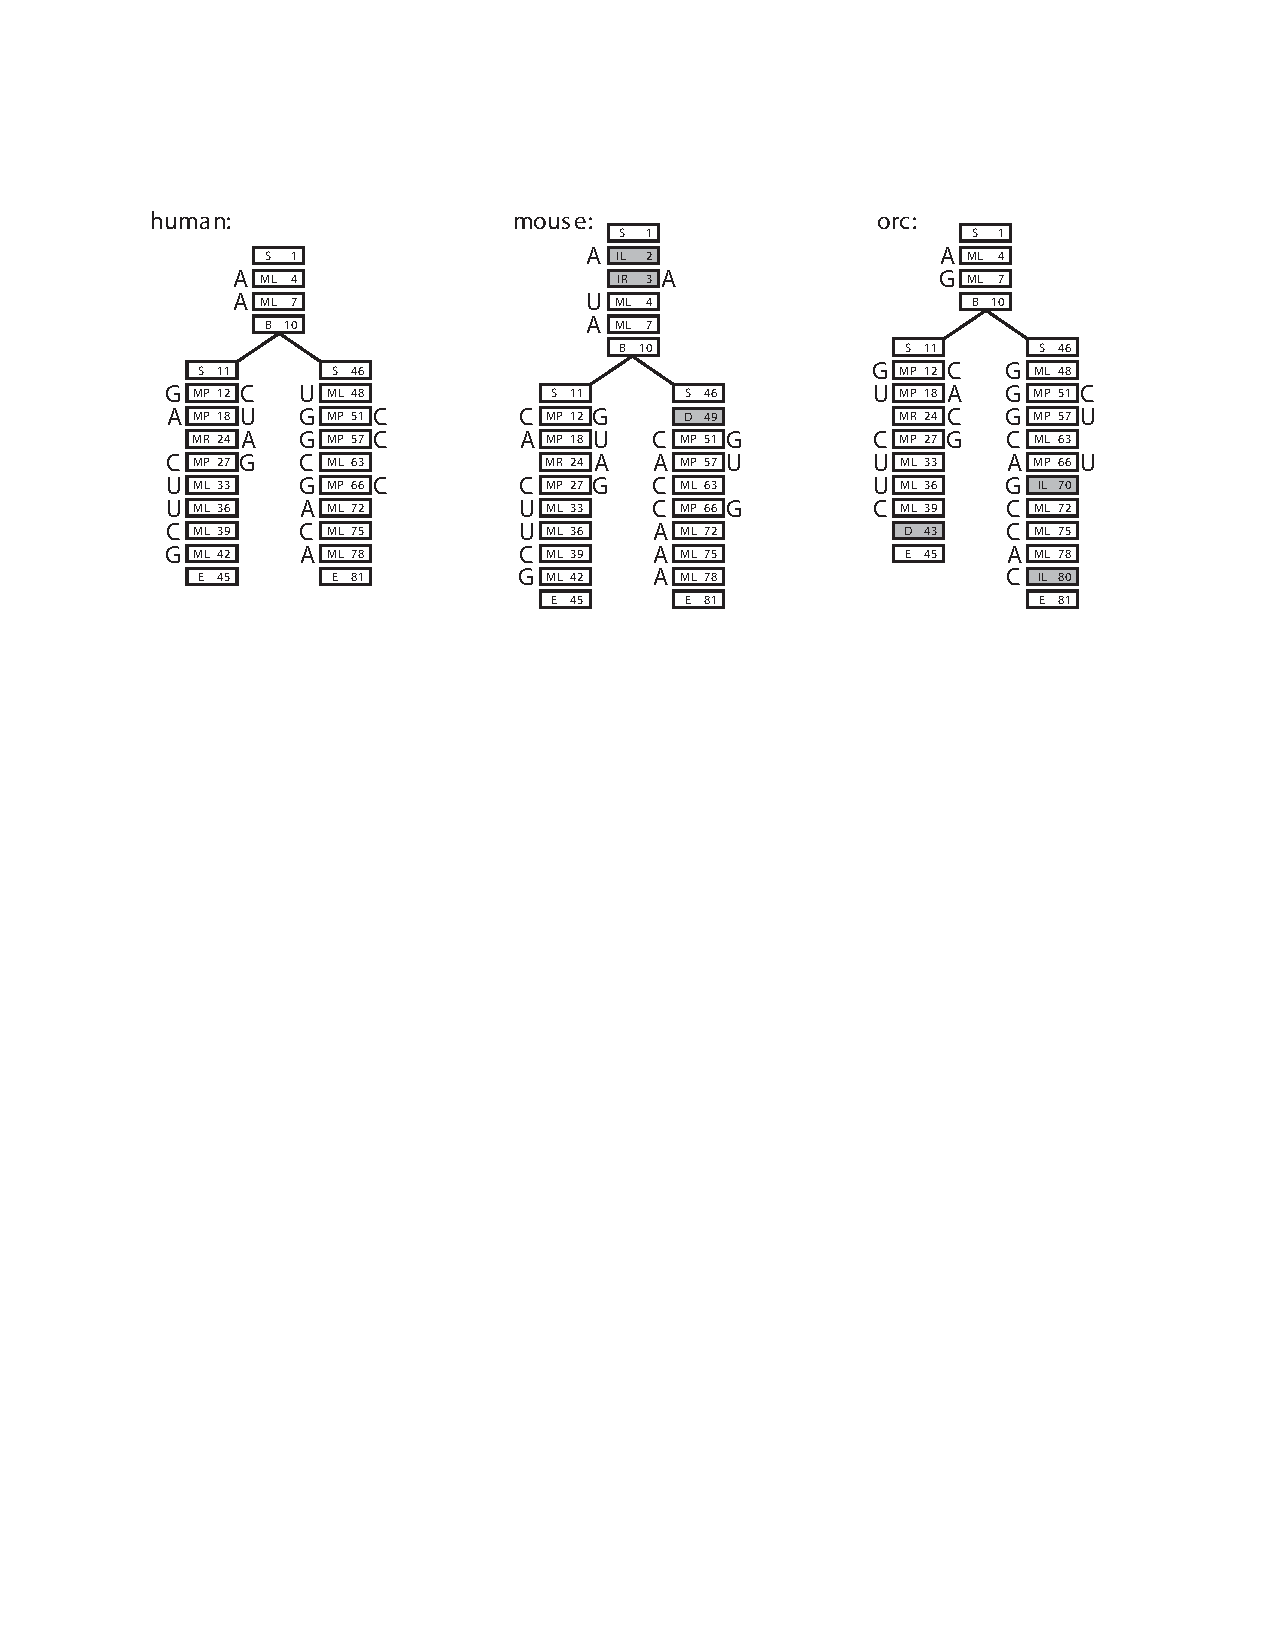
\includegraphics[width=5in]{Figures/parsetrees}
\end{center}
\caption{\small\textbf{Example parse trees.} Parse trees are shown for the
three sequences/structures from Figure~\ref{fig:input_alignment},
given the CM in Figure~\ref{fig:cm_graph}. For each sequence, each
residue must be associated with a state in the parse tree. (The
sequences can be read off its parse tree by starting at the upper left
and reading counterclockwise around the edge of parse tree.) Each
parse tree corresponds directly to a secondary structure -- base pairs
are pairs of residues aligned to MP states. A collection of parse
trees also corresponds to a multiple alignment, by aligning residues
that are associated with the same state -- for example, all three
trees have a residue aligned to state ML4, so these three residues
would be aligned together. Insertions and deletions relative to the
consensus use nonconsensus states, shown in gray.}
\label{fig:parsetrees}
\end{figure}

\subsubsection{Comparison to profile HMMs}

The relationship between an SCFG and a covariance model is analogous
to the relationship of hidden Markov models (HMMs) and profile HMMs
for modeling multiple sequence alignments
\cite{Krogh94,Durbin98,Eddy98}. A comparison may be instructive to
readers familiar with profile HMMs.  A profile HMM is a repetitive HMM
architecture that associates each consensus column of a multiple
alignment with a single type of model node -- a MATL node, in the
above notation. Each node contains a ``match'', ``delete'', and
``insert'' HMM state -- ML, IL, and D states, in the above notation.
The profile HMM also has special begin and end states. Profile HMMs
could therefore be thought of as a special case of CMs. An
unstructured RNA multiple alignment would be modeled by a guide tree
of all MATL nodes, and converted to an unbifurcated CM that would
essentially be identical to a profile HMM. (The only difference is
trivial; the CM root node includes a IR state, whereas the start node
of a profile HMM does not.) All the other node types (especially MATP,
MATR, and BIF) and state types (e.g. MP, MR, IR, and B) are SCFG
augmentations necessary to extend profile HMMs to deal with RNA
secondary structure.


\subsection{The \prog{cmbuild} program, step by step}
%\addtocontents{faq}{\textbf{Questions about using cmbuild:}}

The \prog{cmbuild} command line syntax is:

\user{cmbuild <options> [cmfile] [alifile]}

where \prog{[alifile]} is the name of the input alignment file, and
\prog{[cmfile]} is the name of the output CM file. What follows
describes the steps that \prog{cmbuild} goes through, and the most
important options that can be chosen to affect its behavior.

\subsubsection{Alignment input file}

The input alignment file must be in Stockholm format, and it must have
a consensus secondary structure annotation line (\verb+#=GC SS_cons+).

The program is actually capable of reading many common multiple
alignment formats (ClustalW, PHYLIP, GCG MSF, and others) but no other
format currently supports consensus RNA secondary structure
annotation. This may change in the future, either when other formats
allow structure annotation, or when \prog{cmbuild} is capable of
inferring consensus structure from the alignment by automated
comparative analysis, as the earlier \software{COVE} suite was capable
of \cite{Eddy94}. 

If the file does not exist, is not readable, or is not in a recognized
format, the program exits with a ``could not be opened for reading''
error. If the file does not have consensus secondary structure
annotation, the program exits with a ``no consensus structure
annotation'' error. This includes all non-Stockholm alignment files.

% EPN, Wed Apr  2 12:47:54 2008, the cat my.sto | cmbuild command
% in this faq no longer works.
\begin{comment}
\begin{srefaq}{Why does \prog{cmbuild} have a \prog{--informat} option, if it only
accepts Stockholm?} If you don't specify \prog{--informat}, the
software has to autodetect the file format. Autodetection of file
formats doesn't work in certain advanced/nonstandard cases, for
instance if you're reading the alignment from standard input instead
of from a file. The \prog{--informat} allows you to override
autodetection; e.g. \prog{cat my.sto | cmbuild --informat Stockholm
my.cm -} is an example of reading the alignment from piped standard
input.
\end{srefaq}
\end{comment}

\subsubsection{Parsing secondary structure annotation}

The structure annotation line only needs to indicate which columns are
base paired to which. It does not have to be in full WUSS notation.
Even if it is, the details of the notation are largely ignored.
Nested pairs of \verb+<>+, \verb+()+, \verb+[]+, or \verb+{}+ symbols
are interpreted as base paired columns. All other columns marked with
the symbols \verb+:,_-.~+ are interpreted as single stranded columns.

A simple minimal annotation is therefore to use \verb+<>+ symbols to
mark base pairs and \verb+.+ for single stranded columns.

If a secondary structure annotation line is in WUSS notation and it
contains valid pseudoknot annotation (e.g.\ additional non-nested
stems marked with AAA,aaa or BBB,bbb, etc.), this annotation is
removed and a warning is printed. \software{infernal} cannot handle
pseudoknots. Internally, these columns are treated as if they were
marked with \verb+.+ symbols.

\begin{srefaq}{How should I choose to annotate pseudoknots?} 
\software{infernal} can only deal with nested base pairs. If there is
a pseudoknot, you have to make a choice of which stem to annotate as
normal nested structure (thus including it in the model) and which
stem to call additional ``pseudoknotted'' structure (thus ignoring it
in the model). For example, for a simple two-stem pseudoknot, should
you annotate it as \verb+AAAA.<<<<aaaa....>>>>+, or
\verb+<<<<.AAAA>>>>....aaaa+?  From an RNA structure viewpoint, which
stem I label as the pseudoknotted one is an arbitrary choice; but
since one of the stems in the pseudoknot will have to be modeled as a
single stranded region by \software{infernal}, the choice makes a
slight difference in the performance of your model. You want your
model to capture as much information content as possible.  Thus, since
the information content of the model is a sum of the sequence
conservation plus the additional information contributed by pairwise
correlations in base-paired positions, you should tend to annotate the
shorter stem as the ``pseudoknot'' (modeling as many base pairs as
possible), and you should also annotate the stem with the more
conserved primary sequence as the ``pseudoknot'' (if one stem is more
conserved at the sequence level, you won't lose as much by modeling
that one as primary sequence consensus only).
\end{srefaq}

If (aside from any ignored pseudoknot annotation) the structure
annotation line contains characters other than \verb+<>()[]{}:_-,.~+
then those characters are ignored (treated as \verb+.+) and a warning
is printed.

If, after this ``data cleaning'', the structure annotation is
inconsistent with a secondary structure (for example, if the number of
\verb+<+ and \verb+>+ characters isn't the same), then the program
exits with a ``failed to parse consensus structure annotation'' error.

\subsubsection{Sequence weighting}

By default, the input sequences are weighted in two ways to compensate
for biased sampling (phylogenetic correlations).  Relative sequence
weights are calculated by the Gerstein/Chothia/Sonnhammer method
\cite{Gerstein94}.  (The \prog{--wgsc} option forces GSC weights, but
is redundant since that's the default.)  To turn relative weighting
off (e.g. set all weights to 1.0), use the \prog{--wnone} option.

Some alignment file formats allow relative sequence weights to be
given in the file. This includes Stockholm format, which has
\verb+#=GS WT+ weight annotations. Normally \prog{cmbuild} ignores any
such input weights.  The \prog{--wgiven} option tells \prog{cmbuild}
to use them.  This lets you set the weights with any external
procedure you like; for example, the \prog{weight} utility program in
\software{squid} implements some common weighting algorithms,
including the fast $O(N)$ Henikoff position-based weights
\cite{Henikoff94b}.

If for some reason you put more than one relative weighting option on
the command line, the last one you give is used.

\begin{srefaq}{Why is \prog{cmbuild} taking so much time?} The GSC weighting algorithm
scales as $O(N^2)$ with the number of sequences $N$. Weighting may
become rate-limiting for \prog{cmbuild} if your alignment contains
many sequences. Model construction itself is fast. You might want to
turn weighting off, or pre-calculate the weights by a faster
algorithm.
\end{srefaq}

Absolute weights (the ``effective sequence number'') is calculate by
``entropy weighting'' \cite{Karplus98}. This sets the balance between
the prior and the data, and affects the information content of the
model. Entropy weighting reduces the effective sequence number (the
total sum of the weights) and increases the entropy (degrading the
information content) of the model until a threshold is reached. The
default entropy is 1.41 bits per position (roughly 0.59 bits of
information, relative to uniform base composition). This threshold can
be changed with the \prog{--ere <x>} option. Entropy weighting may
be turned off entirely with the \prog{--enone} option.


\subsubsection{Architecture construction}

The CM architecture is now constructed from your input alignment and
your secondary structure annotation, as described in the previous
section. 

The program needs to determine which columns are consensus (match)
columns, and which are insert columns. (Remember that although WUSS
notation allows insertions to be annotated in the secondary structure
line, \prog{cmbuild} is only paying attention to annotated base
pairs.) By default, it does this by a simple rule based on the
frequency of gaps in a column. If the frequency of gaps is greater
than a threshold, the column is considered to be an insertion. 

The threshold defaults to 0.5. It can be changed to another number
\verb+<x>+ (from 0 to 1.0) by the \prog{--gapthresh <x>} option.  The
higher the number, the more columns are included in the model.  At
\prog{--gapthresh 1.0}, all the columns are considered to be part of
the consensus. At \prog{--gapthresh 0.0}, only columns with no gaps are.

You can also manually specify which columns are consensus versus
insert by including reference coordinate annotation (e.g. a
\verb+#=GC RF+ line, in Stockholm format) and using the \prog{--rf}
option. Any columns marked by non-gap symbols become consensus
columns. (The simplest thing to do is mark consensus columns with x's,
and insert columns with \verb+.+'s. Remember that spaces aren't
allowed in alignments in Stockholm format.) If you set the \prog{--rf}
option but your file doesn't have reference coordinate annotation, the
program exits with an error.

\subsubsection{Parameterization}

Weighted observed emission and transition counts are then collected
from the alignment data. These count vectors $c$ are then converted to
estimated probabilities $p$ using mixture Dirichlet priors. The
default mixture priors are described in \cite{NawrockiEddy07}. You can
provide your own prior as a file, using the \prog{--priorfile <f>}
option.

\subsubsection{Naming the model}

Each CM gets a name. Stockholm format allows the alignment to have a
name, provided in the \verb+#=GF ID+ tag. If this name is provided,
it is used as the CM name.

Stockholm format allows more than one alignment per file, and
\prog{cmbuild} supports this: CM files can contain more than one
model, and if you say e.g.\ \prog{cmbuild Rfam Rfam.sto} where
\verb+Rfam.sto+ contains a whole database of alignments,
\prog{cmbuild} will create a database of CMs in the \verb+Rfam+ file,
one per alignment. 

If a name or names are not provided in the Stockholm \verb+#=GF ID+
annotation, the name given to each CM is the input filename plus a ``-''
character and an integer indicating the position of that alignment
within the alignment file. For example, if you build a model from a
single alignment in alignment file \verb+RNaseP.sto+, the model will
be named RNaseP-1. 

If the \prog{--cmaxid, --ctarget} or \prog{--call} options are used to
split each input alignment into several alignments (see the
``Tutorial'' for an example), then an additional extension of ``.''
plus an integer indicating the order in which the model was
constructed from the alignment is added to the name. For example, if
you run \prog{cmbuild --ctarget 3} with from a the alignment file
\verb+RNaseP.sto+, \prog{cmbuild} will cluster the alignment by
sequence identity into 3 clusters and build 3 CMs, one from each
cluster. These CMs will be named: RNaseP-1.1, RNaseP-1.2 and RNaseP-1.3.

If the alignment file only has 1 alignment in it, you can override the
automatic naming conventions and provide your own name with the \prog{-n <s>}
option, where \verb+<s>+ is any string. 

\subsubsection{Saving the model}

The model is now saved to a file, according to the filename specified
on the command line. By default, a new file is created, and the model
is saved in a portable ASCII text format.

If the cmfile already exists, the program exits with an error. The
\prog{-F} option causes the new model to overwrite an existing
cmfile. The \prog{-A} option causes the new model to be appended to
an existing cmfile (creating a growing CM database, perhaps).

